\chapter{$\gamma$-Astronomie} 
Die Astronomie ist die Wissenschaft des Universums und beschreibt die Bewegung und Eigenschaften von Himmelskörpern wie Planeten oder Galaxien, interstellarer Materie und Strahlung. Betrachtete man früher nur Licht im optisch sichtbaren Bereich, so sind im 20. Jahrhundert einige zusätzliche Quellen dazugekommmen. Dazu zählen die von Viktor Hess durch Ballonversuche entdeckte kosmische Strahlung, die Röntgen-/bzw die Gammastrahlung sowie die Neutrinoastronomie. Die $\gamma$-Astronomie beschäftigt sich mit Photonen im Bereich ab einer Energie von 100 GeV \cite{DesignConcept}. Photonen haben den Vorteil, dass sie nicht wie geladene Teilchen durch elektromagnetische Felder abgelenkt werden und somit ihre Quelle leichter detektiert werden kann. Zudem sind sie auch noch deutlich leichter zu detektieren sind als Neutrinos. Da die Energie dieser Gammastrahlung so hoch ist, können sie nicht thermischen Ursprungs sein sondern kommen aus anderen Quellen, deren Untersuchung das Ziel der Hochenergie-Gamma-Astronomie (VHE - Very High Energy) ist.

\section{Entstehung hochenergetischer Strahlung}

\begin{description}
\item[inverser Comptoneffekt]\hfill \\
Durch den Comptoneffekt können hochenergetische Photonen einen Teil ihres Impulses und Energie an ein freies Elektron übergeben. Dieser Prozess kann auch invers ablaufen und somit kann ein niederenergetisches Photon, zum Beispiel aus dem kosmischen Mikrowellenhintergrund (E=66meV), durch einen Stoß mit einem Elektron eine hohe Energie bekommen.
\item[Bremstrahlung]\hfill \\
Durchfliegen hochenergetische Teilchen Materie, so kann es vorkommen, dass diese eng an den Atomen vorbeifliegen und abgelenkt werden. Durch diese Ablenkung werden Photonen abgestrahlt.
\item[Zerfälle und Annihilation]\hfill \\ 
Hochenergetische Photonen können auch durch Zerfälle massiver Teilchen entstehen, wobei die Ruhemasse des Teilchen in kinetischer Energie der Photonen umgewandelt wird. So zerfällt das neutrale Pion zum Beispiel zu 98,8\% \cite{PDG} in zwei Photonen und setzt dabei eine Ruhemasse von $E_0=135MeV$ \cite{PDG} um. Eine weitere Möglichkeit ist die Annihilation von Materie und Antimaterie. Auch hier wird die Ruheenergie der Teilchen in kinetische Energie umgewandelt. So entstehen bei der Elektron-Positron-Annihilation zwei Photonen mit der Energie $E=511keV$.
Diese Energien liegen allerdings noch weit unter der Grenze der VHE.

\end{description}

\section{Quellen hochenergetischer Strahlung}
Ziel VHE-Astronomie ist es die Quellen hochenergetischer Gammastrahlung zu erforschen.

\begin{description}
\item[Supernova Überreste]\hfill \\
Hat ein Stern mit ausreichender Masse seinen Wasserstoff- und Heliumvorrat verbrannt und somit sein Lebensende erreicht, kollabiert dieser und es entsteht ein kompaktes Objekt, wie zum Beispiel ein Neutronenstern, der mit der ihn umgebenden Materie interagieren kann.
\item[Schwarze Löcher]\hfill \\
Schwarze Löcher sind Objekte mit einer Gravitationskraft, die so stark ist, dass auch Photonen, die sich hinter dem Ereignishorizont befinden nicht entkommen können. Durch die starke Anziehung entsteht eine Akkretionsscheibe in der große elektromagnetische Felder herrschen, durch die wiederum hochenergetische Photonen entstehen können.
\item[Aktive Galaxien und aktive galaktische Kerne]\hfill \\
Da schwarze Löcher zu den hellsten Gammaquellen gehören und sich in der Regel im Zentrum einer Galaxie befinden, können diese überstrahlen. Häufig werden diese als stellare Objekte wargenommen. AGNs haben eine Masse von rund 100 Millionen Sonnenmassen. Zu den AGNs gehören auch Blazare und Quasare.
\item[Pulsare]\hfill \\
Kollabieren die Überreste einer Supernova von einem Durchmesser von ca $10^6km$ auf ca $20km$ ensteht ein Neutronenstern, der sich aufgrund der Drehimpulserhaltung sehr schnell dreht. Solche Konstrukte nennt man Pulsare. Bleibt der magnetische Fluss durch die Oberfläche erhalten, entstehen große Magnetfelder ($\mathcal{O}(10^8\unit{T})$\cite{Grupen}. In diesem rotierenden Magnetfeld können geladene Teilchen durch die Lorentzkraft auf hohe Geschwindigkeiten beschleunigt werden, die ihre Energie wiederum an Photonen abgeben können.
\item[Binäre Systeme]\hfill \\ 
Befindet sich ein Neutronenstern oder Pulsar in einem System mit einem normalen Stern, entsteht durch Absaugen von Materie eine Akkretionsscheibe um den Neutronenstern beziehungsweise um den Pulsar. Durch diese Plasmabewegungen entstehen elektromagnetische Felder, in denen Teilchen Energien in der Größenordnung $10^{19} \unit{eV}$\cite{Grupen} erhalten.
\item[Dunkle Materie]\hfill \\
Da die VHE-Astronomie sich mit Energien beschäftigt, die in keinem Experiment auf der Erde realisiert werden können, erhofft man sich auch Erkenntnisse zu ungeklärten Fragen der Physik, wie zum Beispiel zur dunklen Materie.
\end{description}


\section{Detektion von Strahlung}
Prinzipiell lässt sich zwischen bodengestützter und satellitengestützter $\gamma$-Astronomie unterscheiden. Durch den Einsatz von Satelliten vermeidet man den störenden Einfluss der Erdatmosphäre, muss dafür allerdings Abstriche in der Größe der Detektoren machen und mit hohen Kosten kalkulieren. Hier soll sich nur mit der bodengestützten Variante beschäftigt werden, die günstiger ist und nicht in der Größe beschränkt ist. Dazu verwendet man sogenannte IACTS (Imaging Atmosphaeric Cherenkov Telescopes), die die Strahlung nur indirekt detektieren.

\subsection{Luftschauer}
Die Atmosphäre ist nur für Photonen im optischen und radio Bereich durchsichtig. Treten hochenergetische Photonen in die Atmosphäre ein, wechselwirken sie mit dieser über Paarbildung. Das entstehende Elektron bzw Positron ist ebenfalls hochenergetisch und verliert hauptsächlich durch Bremstrahlung Energie, worauf die entstehenden Photonen wieder durch Paarbildung wechselwirken können. Die Strahlungslängen für Paarbildung und Bremsstrahlung sind ungefähr gleich lang, sodass die Anzahl der Teilchen mit absteigender Höhe exponentiell zunimmt, wohingegend die durchschnittliche Energie der Teilchen exponentiell abnimmt. Der Luftschauer endet, in einer Höhe von ungefähr 10km 
\cite{iwas}, wenn die Teichen niederenergetisch sind und die restliche Energie über Ionisation verlieren.
\begin{equation}
E_n=\frac{E_0}{2^n}
\end{equation}\\
Neben den oben beschriebenen elektromagnetischen Schauern existieren noch hadronische und myonische Schauer. Hadronische Schauer entstehen wenn hochenergetische Hadronen in die Atmosphaere eindringen. Durch die Wechselwirkung von Hadronen entstehen haufig Pionen, die wiederum in Photonen zerfallen, wodurch wiederum ein elekromagnetischer Schauer entsteht, der allderdings einen anderen Ursprung hat. Entstehen Myonen in einem Schauer, so besteht das Problem, dass diese kaum Energie abgeben und bei hoher Geschwindigkeit den Erdboden erreichen. Somit gibt nur ein Teil des Schauers die Energie ab und die Messung weicht von der Realität ab.

\subsection{Cherenkov Strahlung}
Cherenkov Strahlung tritt auf, wenn geladene sich Teilchen in Materie schneller als die Lichtgeschwindigkeit in diesem Medium bewegen. Hierbei polarisiert das geladene Teilchen auf seiner Trajektorie die einzelnen Atome, die Licht sphärisch abstrahlen. Wäre das Teilchen langsamer als die Ausbreitungsgeschwindigkeit in diesem Medium, würden die Wellen destruktiv interferrieren und man würde keine makroskopischen Effkte beobachten. Da sich das Teilchen allerdings schneller als das Licht bewegt, entsteht ein Kegel konstruktiver Interferenz, und ein Lichtblitz breitet sich kegelförmig mit dem Oeffnungswinkel
\begin{equation}
\theta = \arccos\left(\frac{1}{\beta n}\right) \label{eq:cherenkow}
\end{equation}\\
aus. Fuer Luft (in Bodennähe) ergibt sich somit ein maximaler Öffnungswinkel von. Da allerdings die Dichte der Luft in der relevanten Höhe kleiner ist, ist auch der Brechungsindex näher an 1 und der Cherenkovwinkel beträgt noch ungefähr $\theta = 1^{\circ}$\cite{Grupen}
\begin{figure}[htbp]
\centering
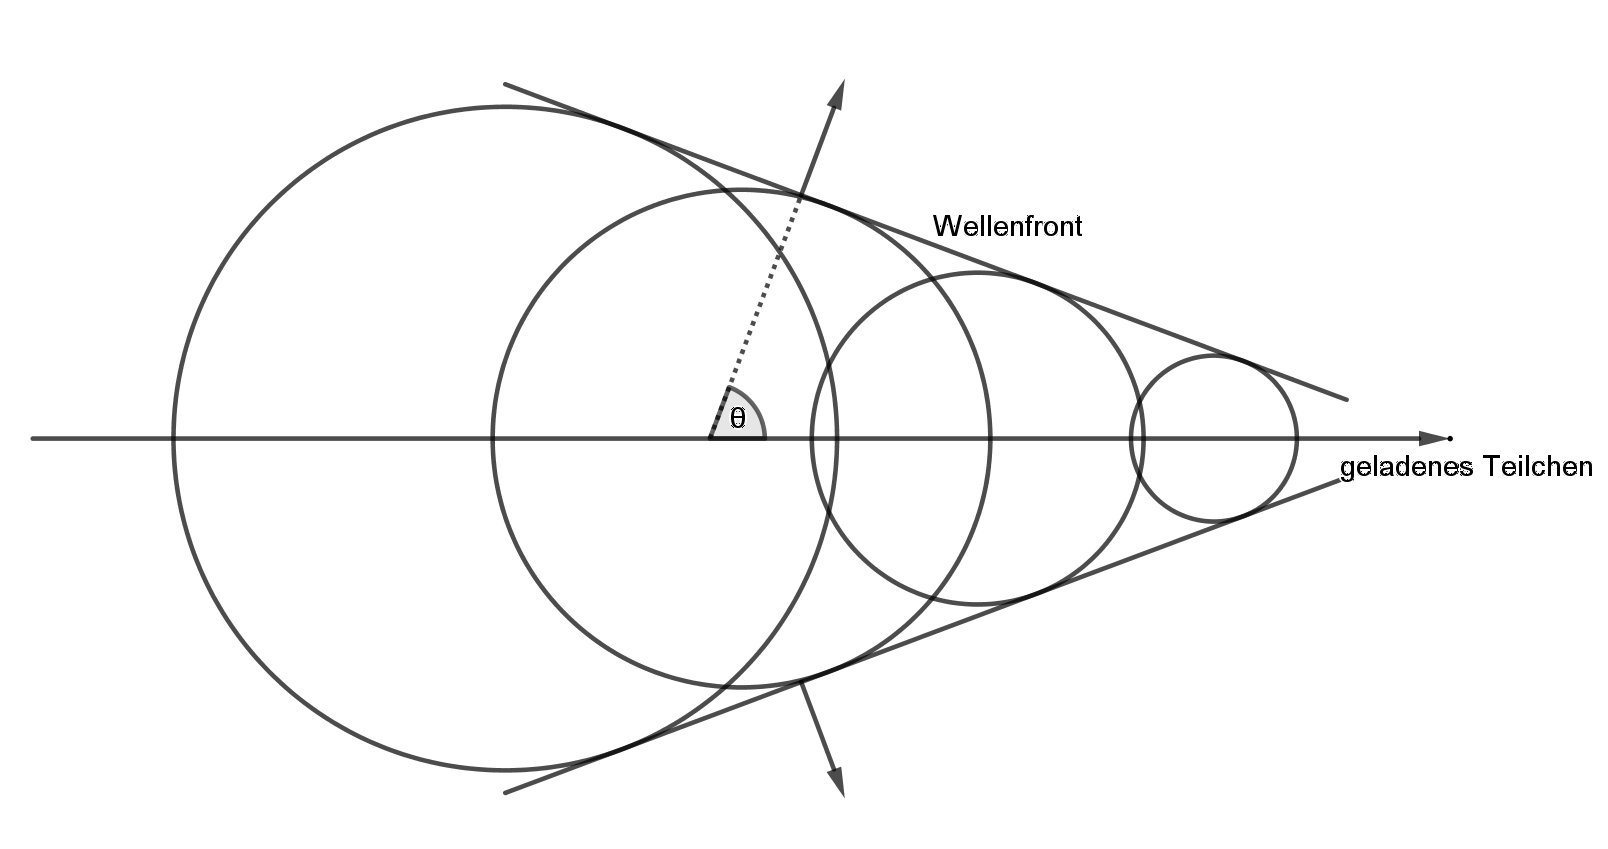
\includegraphics[width=0.7\textwidth]{Images/cherenkow.png}
\caption{Der Cherenkoweffekt: Ein geladenes Teilchen durchfliegt ein dielektrisches Medium mit einer Geschwindigkeit über der der Lichtgeschwindigkeit im Medium und erzeugt Wellenfronten.}
\label{img:cherenkow}
\end{figure}
Aus dem Winkel lässt sich die Geschwindigkeit des Teilchens rekonstruieren und bei bekannter Masse des Teilchens (in elektromagnetischen Schauern entstehen Elektronen als geladene Teilchen) auch der Impuls und die Energie.

\subsection{Bodengestützte Detektion der Cherenkovstrahlung}
Ziel der bodengestützten Variante ist es das Cherenkovlicht der sekundären Teilchen aus dem elektromagnetischen Schauer zu detektieren. Bei einem Cherenkovwinkel von $\theta=1^\{circ}$ in 10km Höhe und senkrechter Einstrahlung ergibt sich ein Lichtpool am Boden mit einem Durchmesser von $250m$ \cite{DesignConcept}. Somit müssen effektive Flächen in der Größenordnung von $10^4$ bis $10^5m^2$ abgedeckt werden um den gesamten Schauer zu detektieren. Typischerweise entstehen bei einem VHE-Photon $10^8-10^9$ Photonen, die innerhalb von wenigen Nanosekunden abgegeben werden. Am Boden hat man somit typische Intenstäten von $10^3\frac{1}{m^2}$ die detektiert werden müssen.
Dazu verwendet man Abbildende Cherenkovteleskope (IACTS - Imaging Atmosphaeric Cherenkov Telescops), die aus einem Reflektor und einem Detektor bestehen. Der Reflektor besteht aus einem oder häufig aus mehreren Spiegeln, die das Cherenkovlicht in der Brennebene bündeln. Bei großen Teleskopen muss der Reflektor parabolisch sein und bei kleineren wird darauf häufig aus Kostengründen verzichtet, da jeder einzelne Spiegel eine individuelle Brennweite braucht.
Als Detektor wird eine Cherenkovkamera verwendet, die eine typische Auflösung von 2000 Pixeln und Zeitaulösung $10ns$\cite{CherenkovCam} hat. Das die Auflösung im Vergleich zu CCD Kameras eher gering ist, liegt daran, dass der Detektor sehr wenige Photonen in einer sehr kurzen Zeit detektiert werden müssen. Dazu verwendet man Photomultiplier.
Aus den aufgenommenen Daten lässt sich mit Hilfe von Monte-Carlo-Simulationen die Richtung und die Energie des detektierten Photons rekonstruieren. 

\begin{figure}[htbp]
\centering
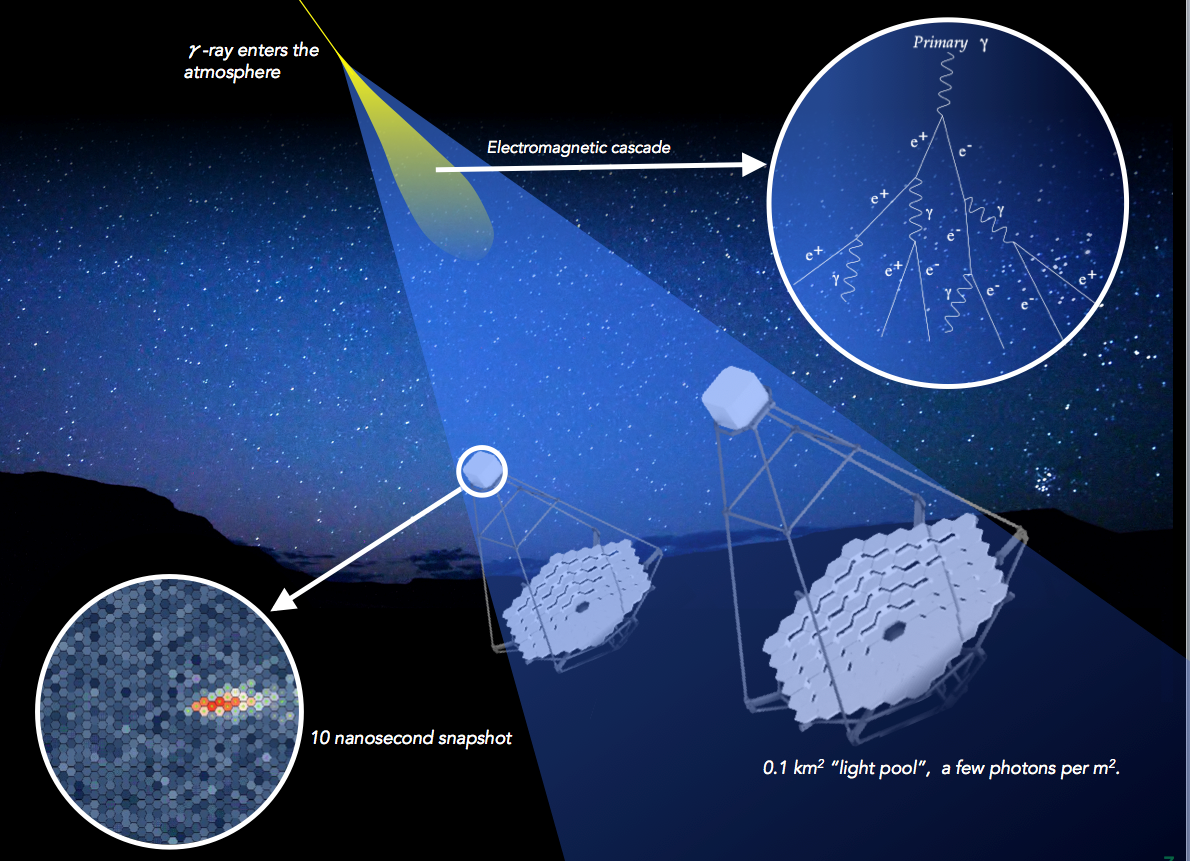
\includegraphics[width=\textwidth]{Images/detection.png}
\caption{Detektion hochenergetischer Strahlung: Das in die Atmosphäre eintretende Photon erzeugt einen elektromagnetischen Luftschauer (oben rechts) der wiederum Cherenkovlicht erzeugt, welches am Boden mit IACTs detektiert werden kann. Ein Detektionsbild ist unten links zu sehen.}
\label{img:detection}
\end{figure}
